%\title{CSCI 440 Check In 2}

\documentclass[10pt]{beamer}

\usetheme[progressbar=frametitle]{metropolis}
\usepackage{appendixnumberbeamer}

\usepackage[compatibility=false]{caption}
\usepackage{subcaption}

\usepackage{booktabs}
\usepackage{hyperref}
\usepackage[scale=2]{ccicons}
\usepackage{tikz}
\usetikzlibrary{positioning}
\usetikzlibrary{3d}
\usepackage{bm}
\usepackage{mathtools}

\usepackage{marvosym}
\usepackage{amssymb}
\usepackage{pifont}

\usepackage{pgfplots}
\usepgfplotslibrary{dateplot}

\usepackage{xspace}
\newcommand{\themename}{\textbf{\textsc{metropolis}}\xspace}

\title{Plasticity and Evolvability}
\subtitle{CSCI 440 Check In 2}
\date{March 20th, 2017}
\author{\texorpdfstring{Matthew Andres Moreno\newline\url{mamoreno@pugetsound.edu}}{Matthew Moreno}}

\titlegraphic{\hfill
\includegraphics[height=2cm]{img/UofPS_stacked_maroonRGB_PNG.png}}

\begin{document}

\maketitle

\section{Evolvability Review}

\begin{frame}{Defining Evolvability}
consensus: the amount of useful variation generated by the evolutionary process
\begin{itemize}
  \item evolvability as the ability to generate heritable variation
  \item evolvability as bias towards useful variation
\end{itemize}
\end{frame}

\begin{frame}{Evolvability as Heritable Variation}
	\begin{figure}
 \centering
    \begin{subfigure}[b]{0.5\textwidth}
        \centering
    	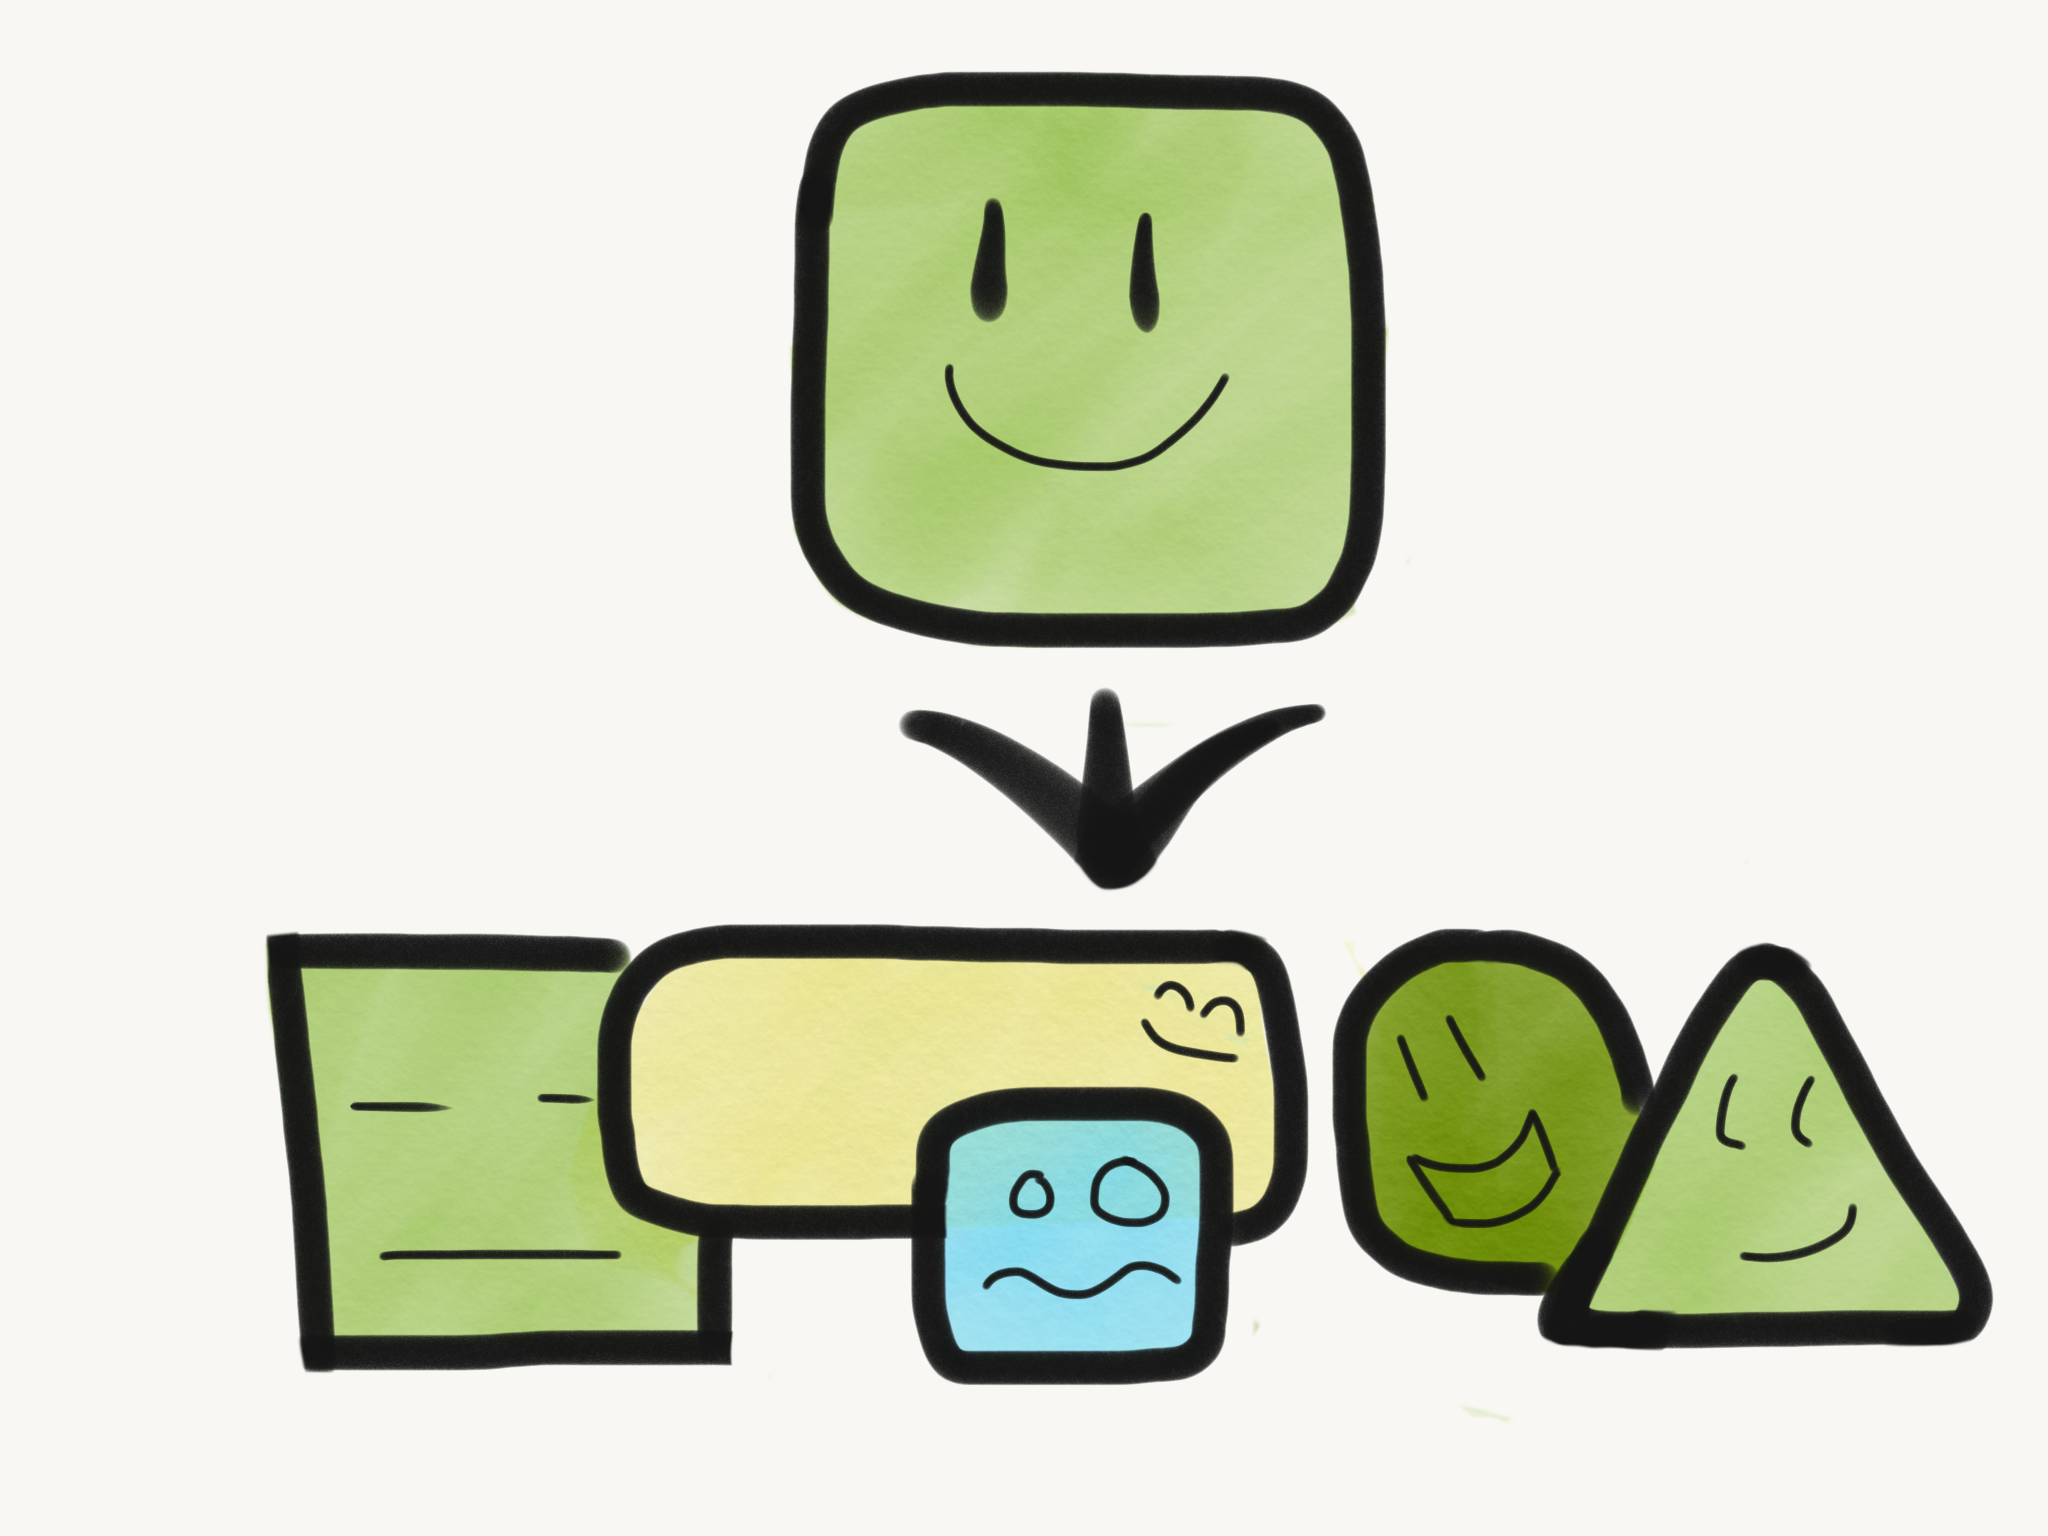
\includegraphics[width=\textwidth]{img/individual_evolvability.png}
        \caption{high individual evolvability}
        \label{subfig:canalization}
    \end{subfigure}%
    \hfill
    \begin{subfigure}[b]{0.5\textwidth}
        \centering
        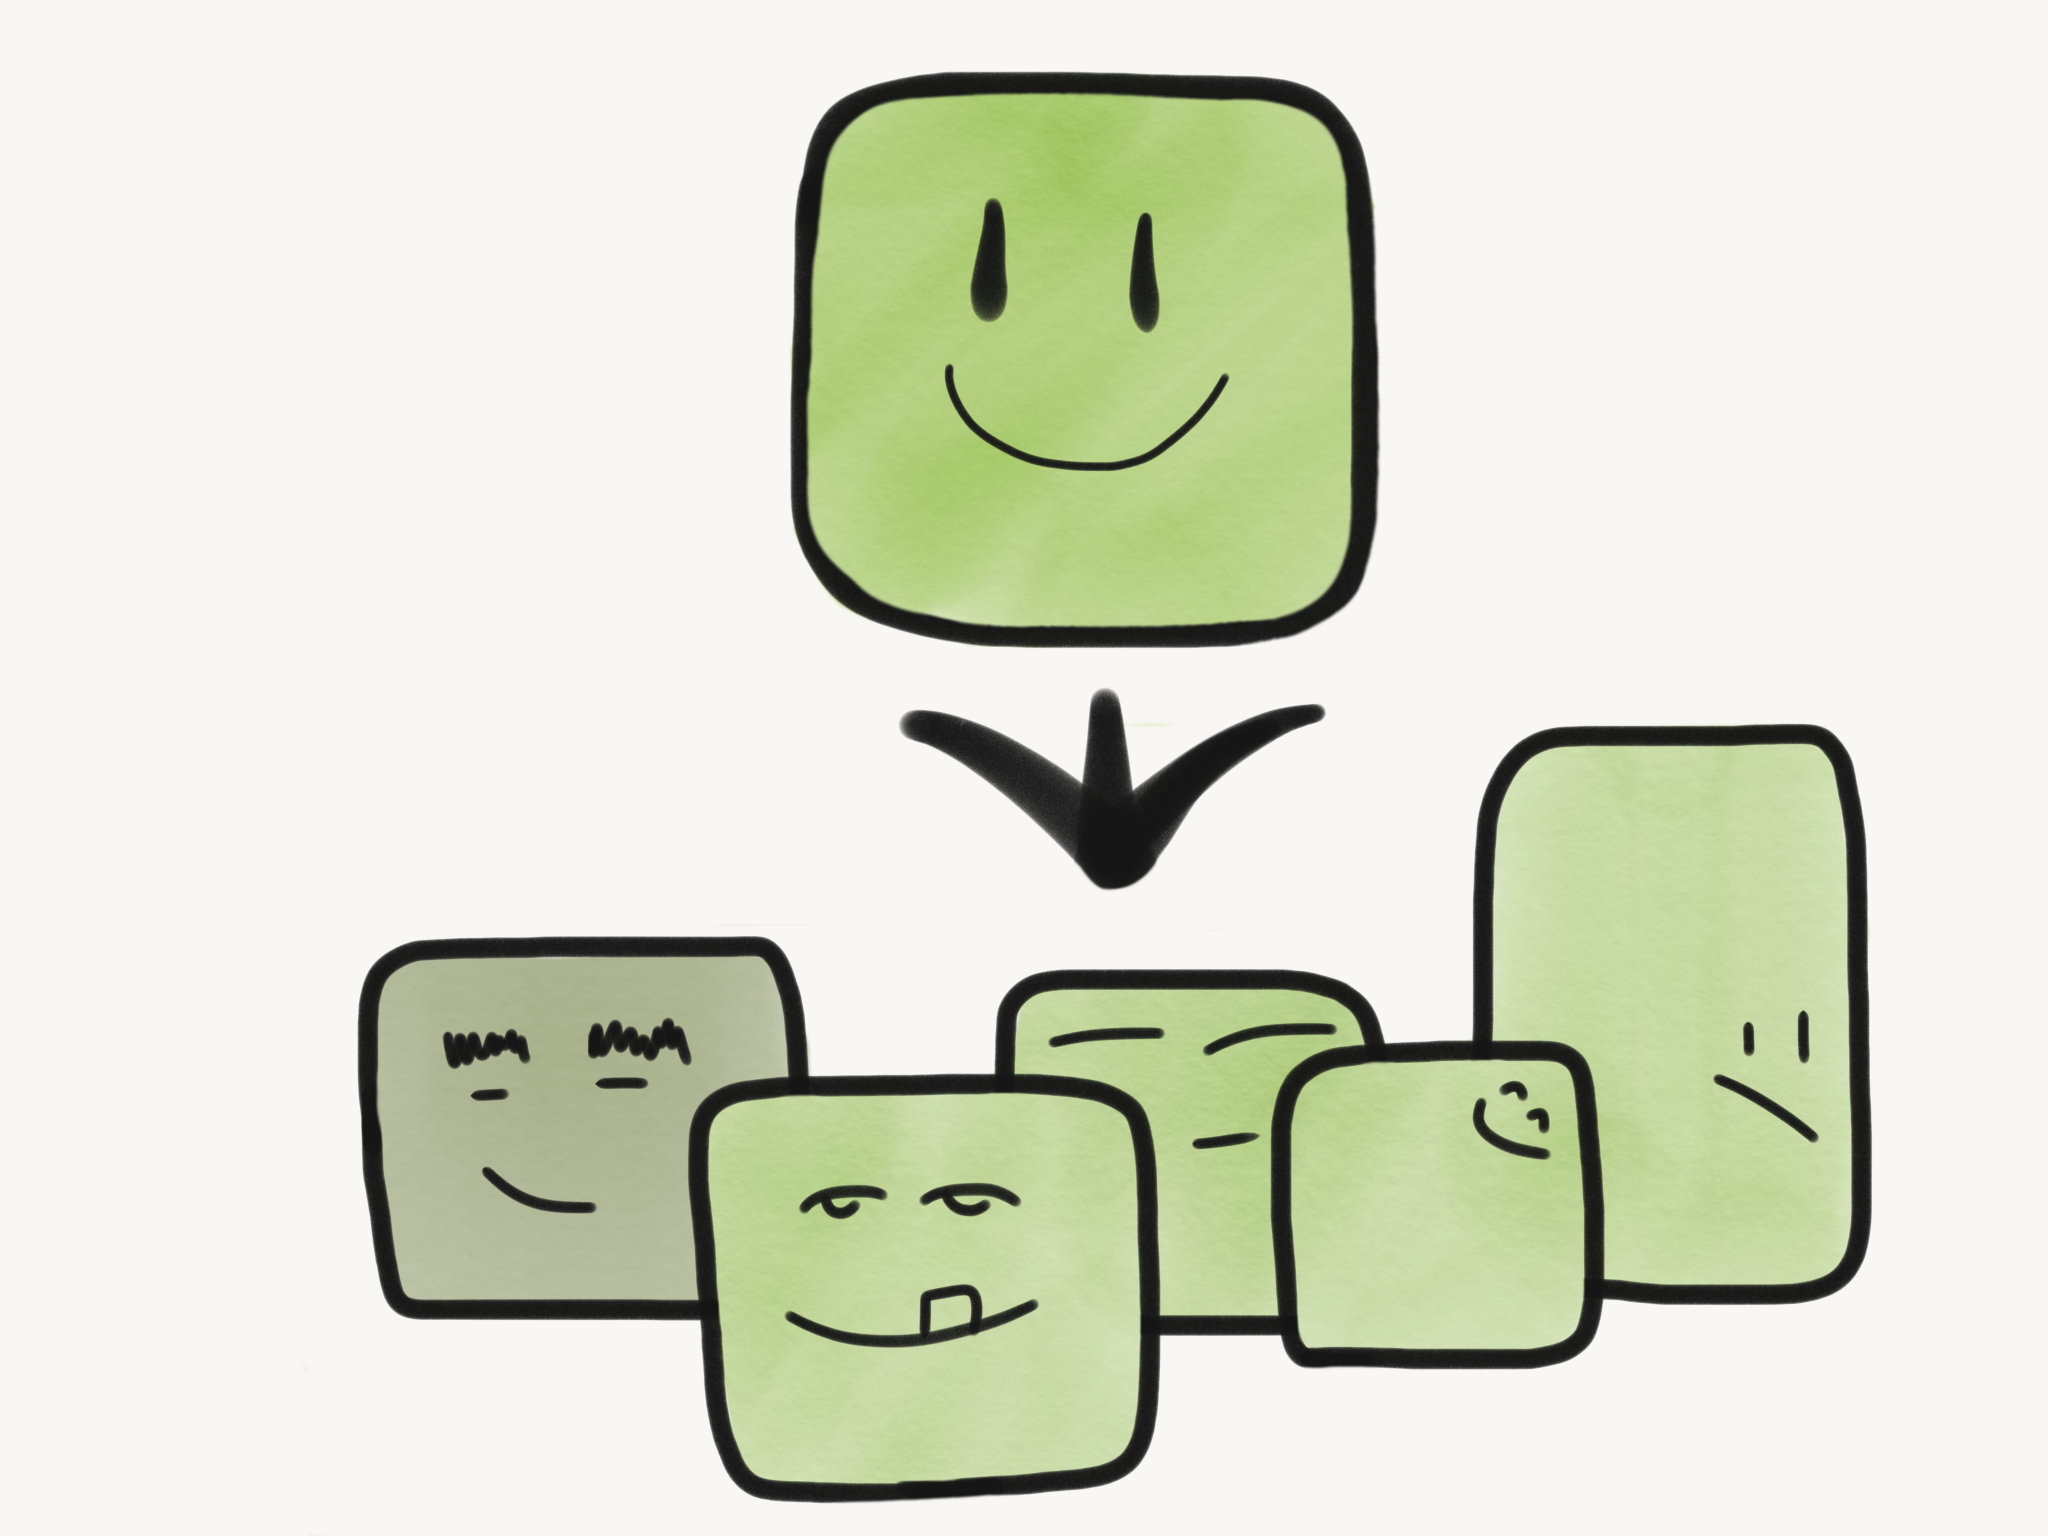
\includegraphics[width=\textwidth]{img/low_individual_evolvability.png}
        \caption{low individual evolvability}
        \label{subfig:no_canalization}
    \end{subfigure}
 	\captionsetup{singlelinecheck=off,justification=raggedright}
    \vspace{-4ex}
  \captionsetup{singlelinecheck=off,justification=raggedright}
  \caption{An illustration of individual evolvability, considering evolvability as heritable variation \cite{Wilder2015ReconcilingEvolvability}.}
  \label{fig:high_vs_low_individual_evolvability}
\end{figure}
\end{frame}

\begin{frame}{Evolvability as Bias towards Useful Variation}
  \begin{figure}
    \centering
    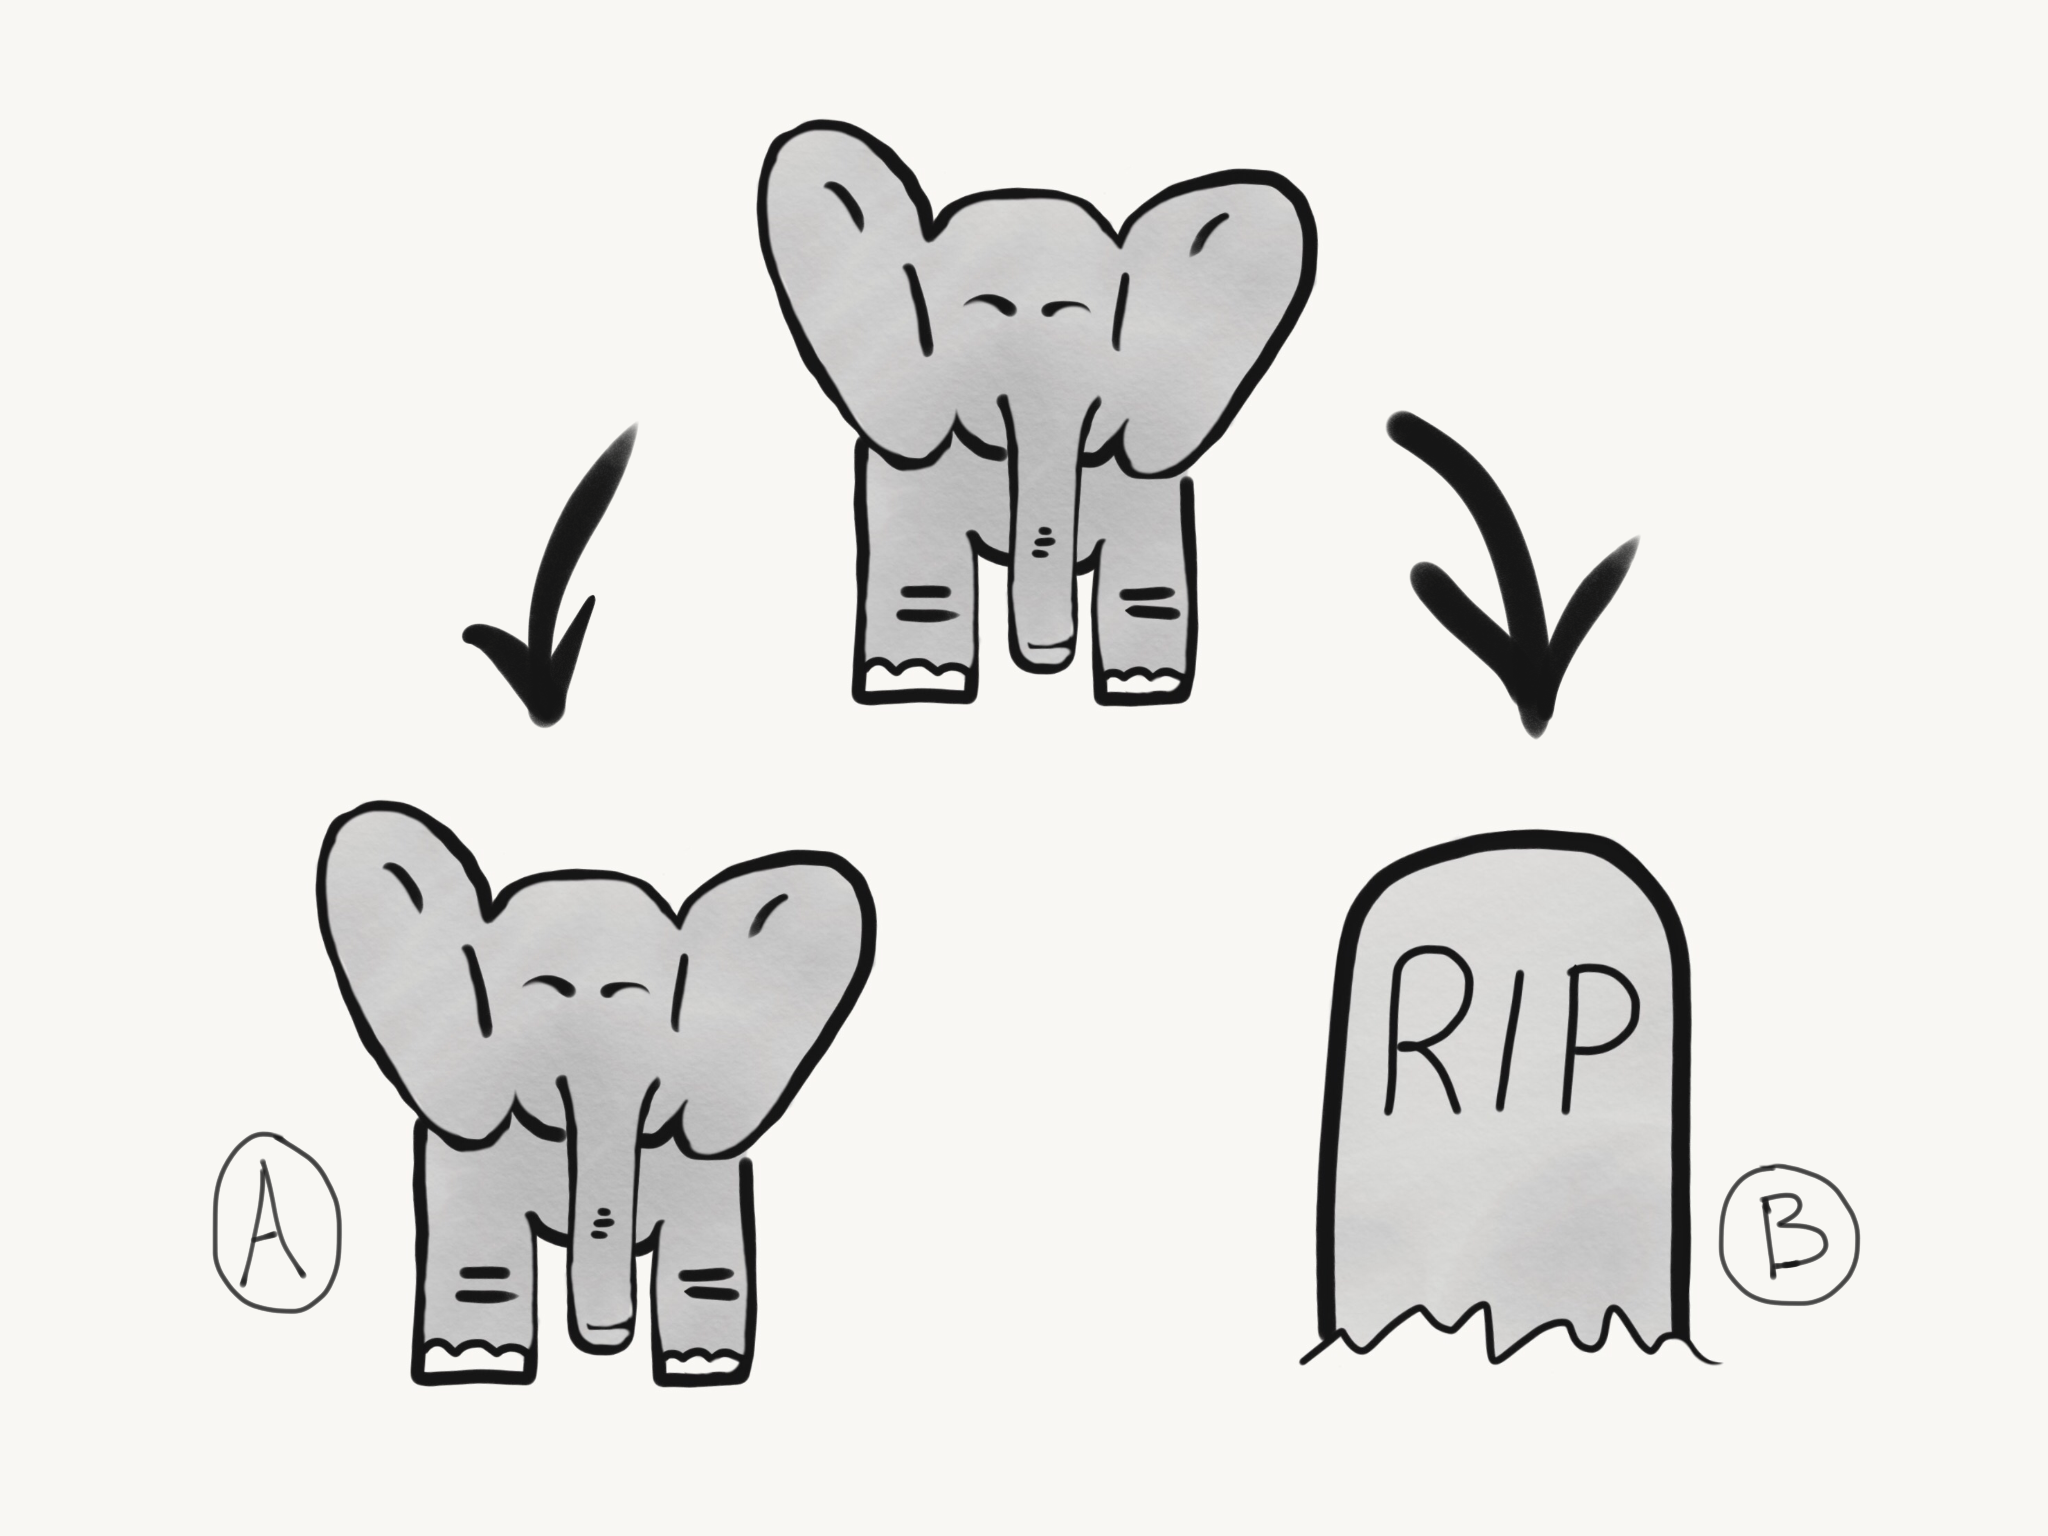
\includegraphics[width=0.8\textwidth]{img/robustness}
 	\captionsetup{singlelinecheck=off,justification=raggedright}
  	\caption{Illustration of robustness; high evolvability left and low evolvability right \cite{Downing2015IntelligenceSystems}.}
    \label{fig:robustness}
\end{figure}
\end{frame}

\begin{frame}{Reading an Evolvability Signature}
  \begin{figure}
  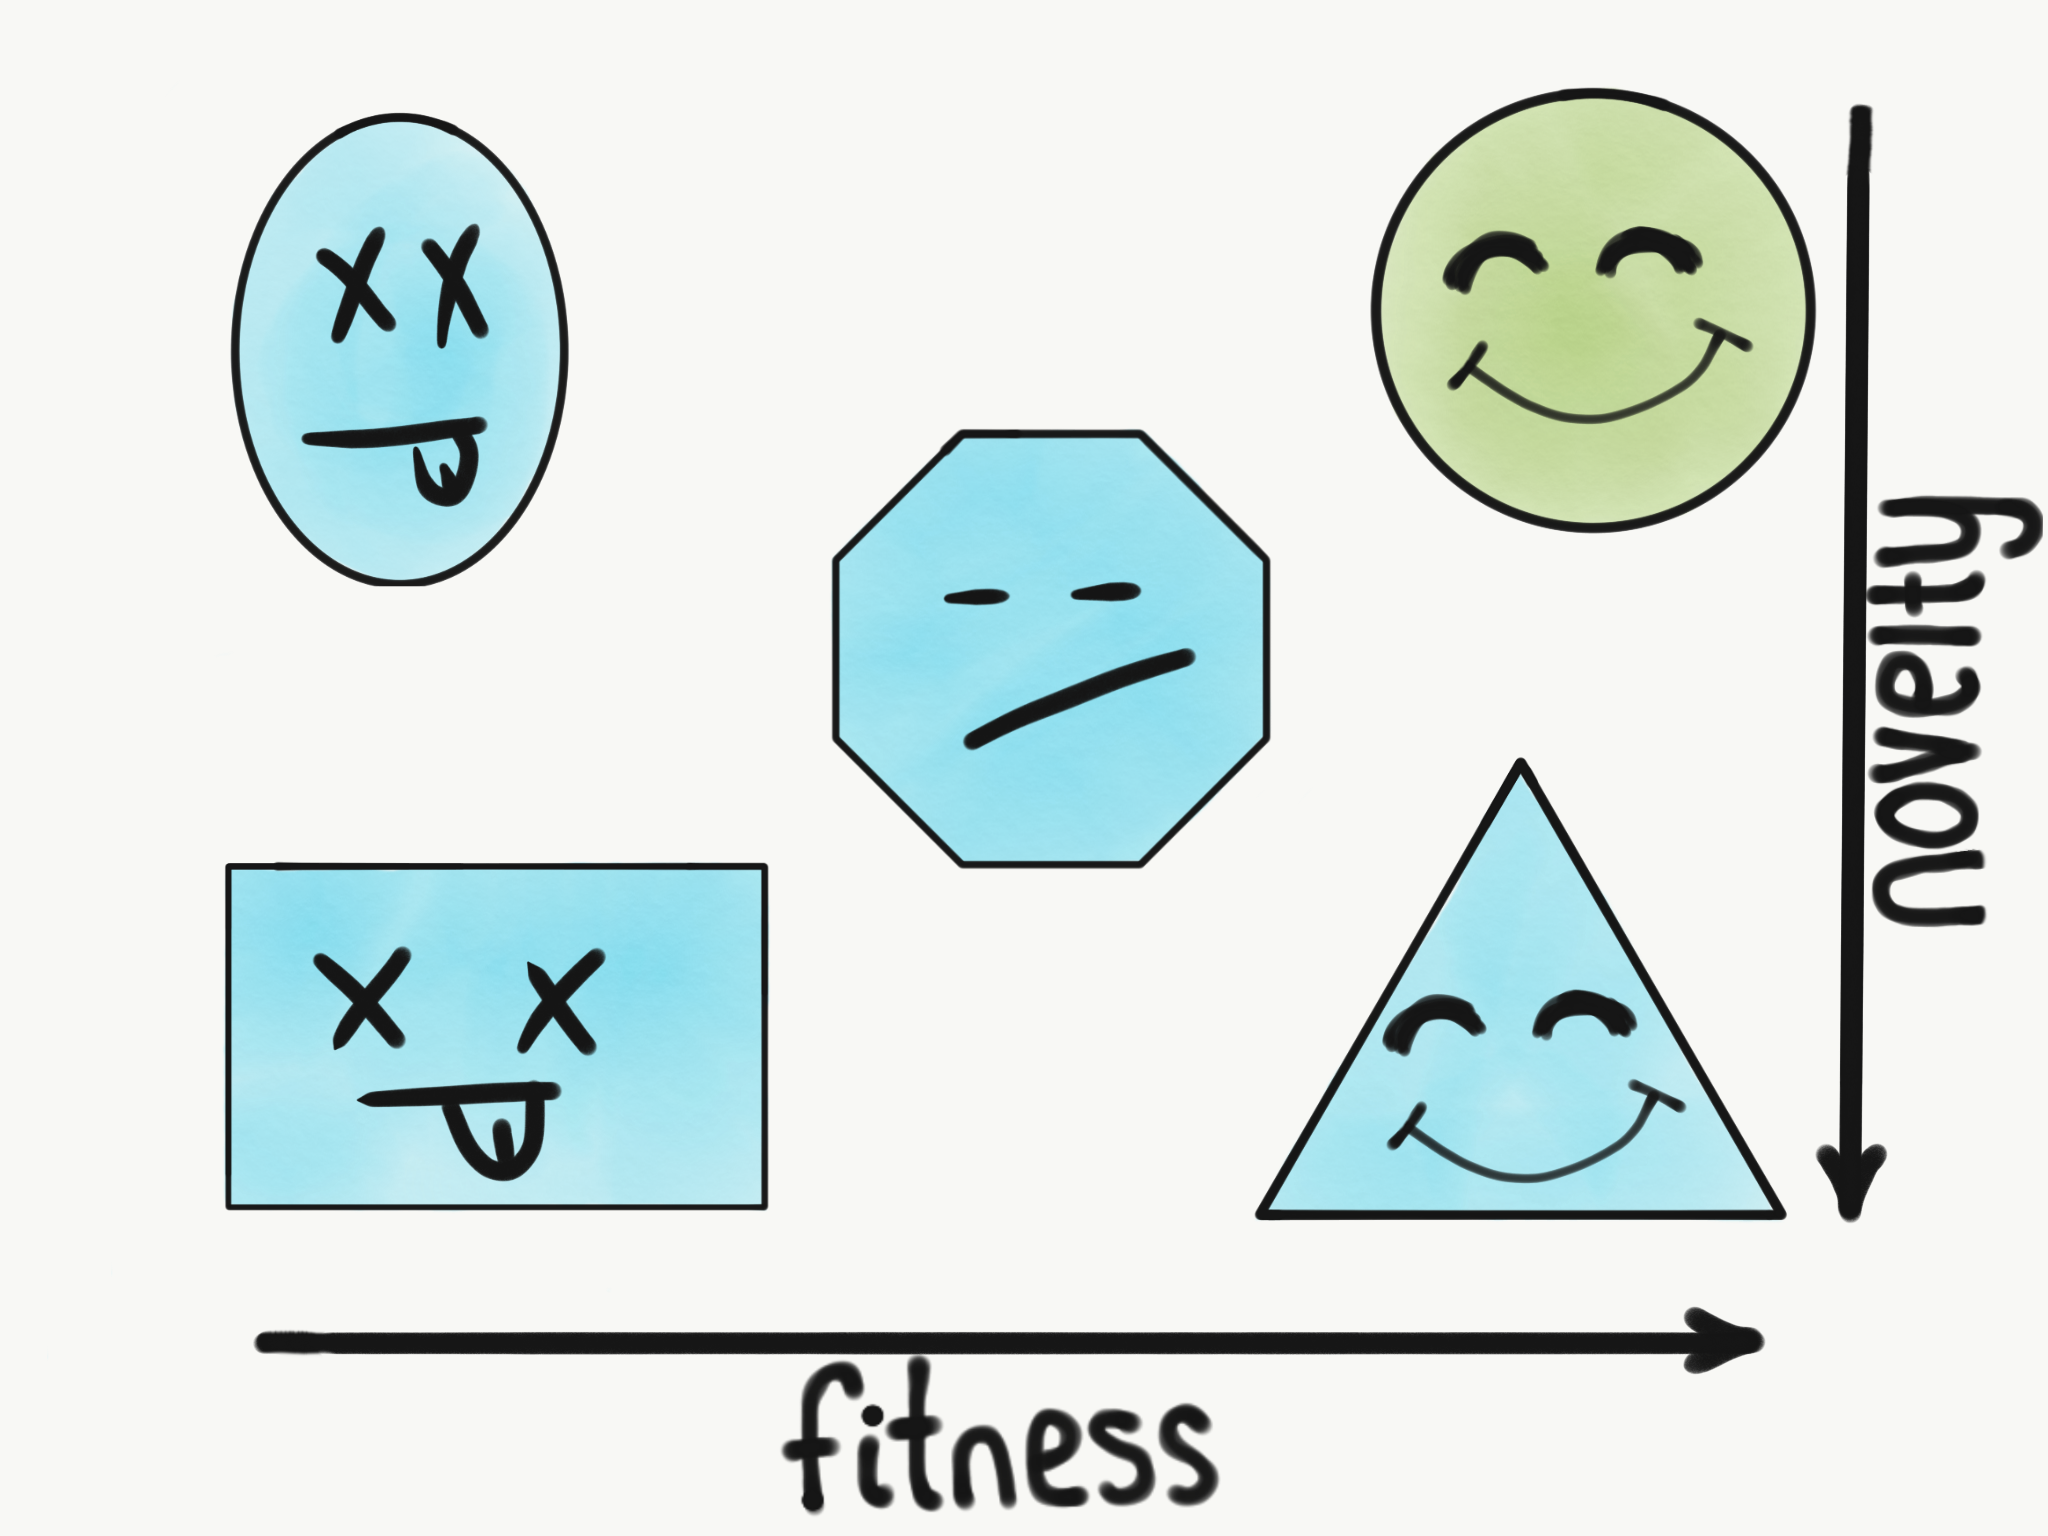
\includegraphics[width=0.8\textwidth]{img/reading_evolvability_signature}
  \captionsetup{singlelinecheck=off,justification=raggedright}
  \caption{Cartoon illustration describing the layout of an evolvability signature diagram \cite{Tarapore2015EvolvabilityBenchmarks}.}
  \label{fig:reading_evolvability_signature}
\end{figure}
\end{frame}


\section{Expanded Model}

\begin{frame}{Motivation}
\begin{itemize}
  \item previous model: phenotypic distance tied directly to fitness score
  \item add more sophisticated fitness evaluation to separate phenotypic distance and fitness score
  \item adjust genetic regulatory network setup to scale better   \item add hidden states to allow greater network intricacy
\end{itemize}
\end{frame}

\begin{frame}{Conway's Game of Life}
\begin{figure}
  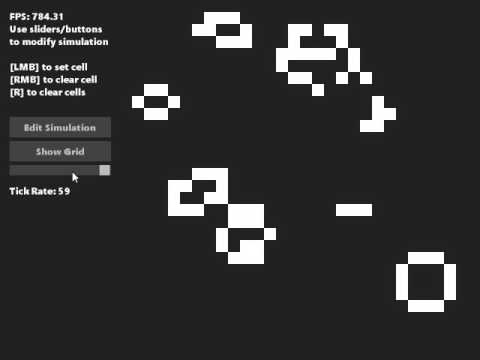
\includegraphics[width=0.8\textwidth]{img/gol_icon}
  \captionsetup{singlelinecheck=off,justification=raggedright}
\href{https://www.youtube.com/watch?v=Kzg5is1lgSk}{\caption{Video illustrations of Conway's Game of Life cellular automata in action.}}
\end{figure}
\end{frame}

\begin{frame}{Adjusted Genetic Regulatory Network Model}
\begin{figure}
    \centering
    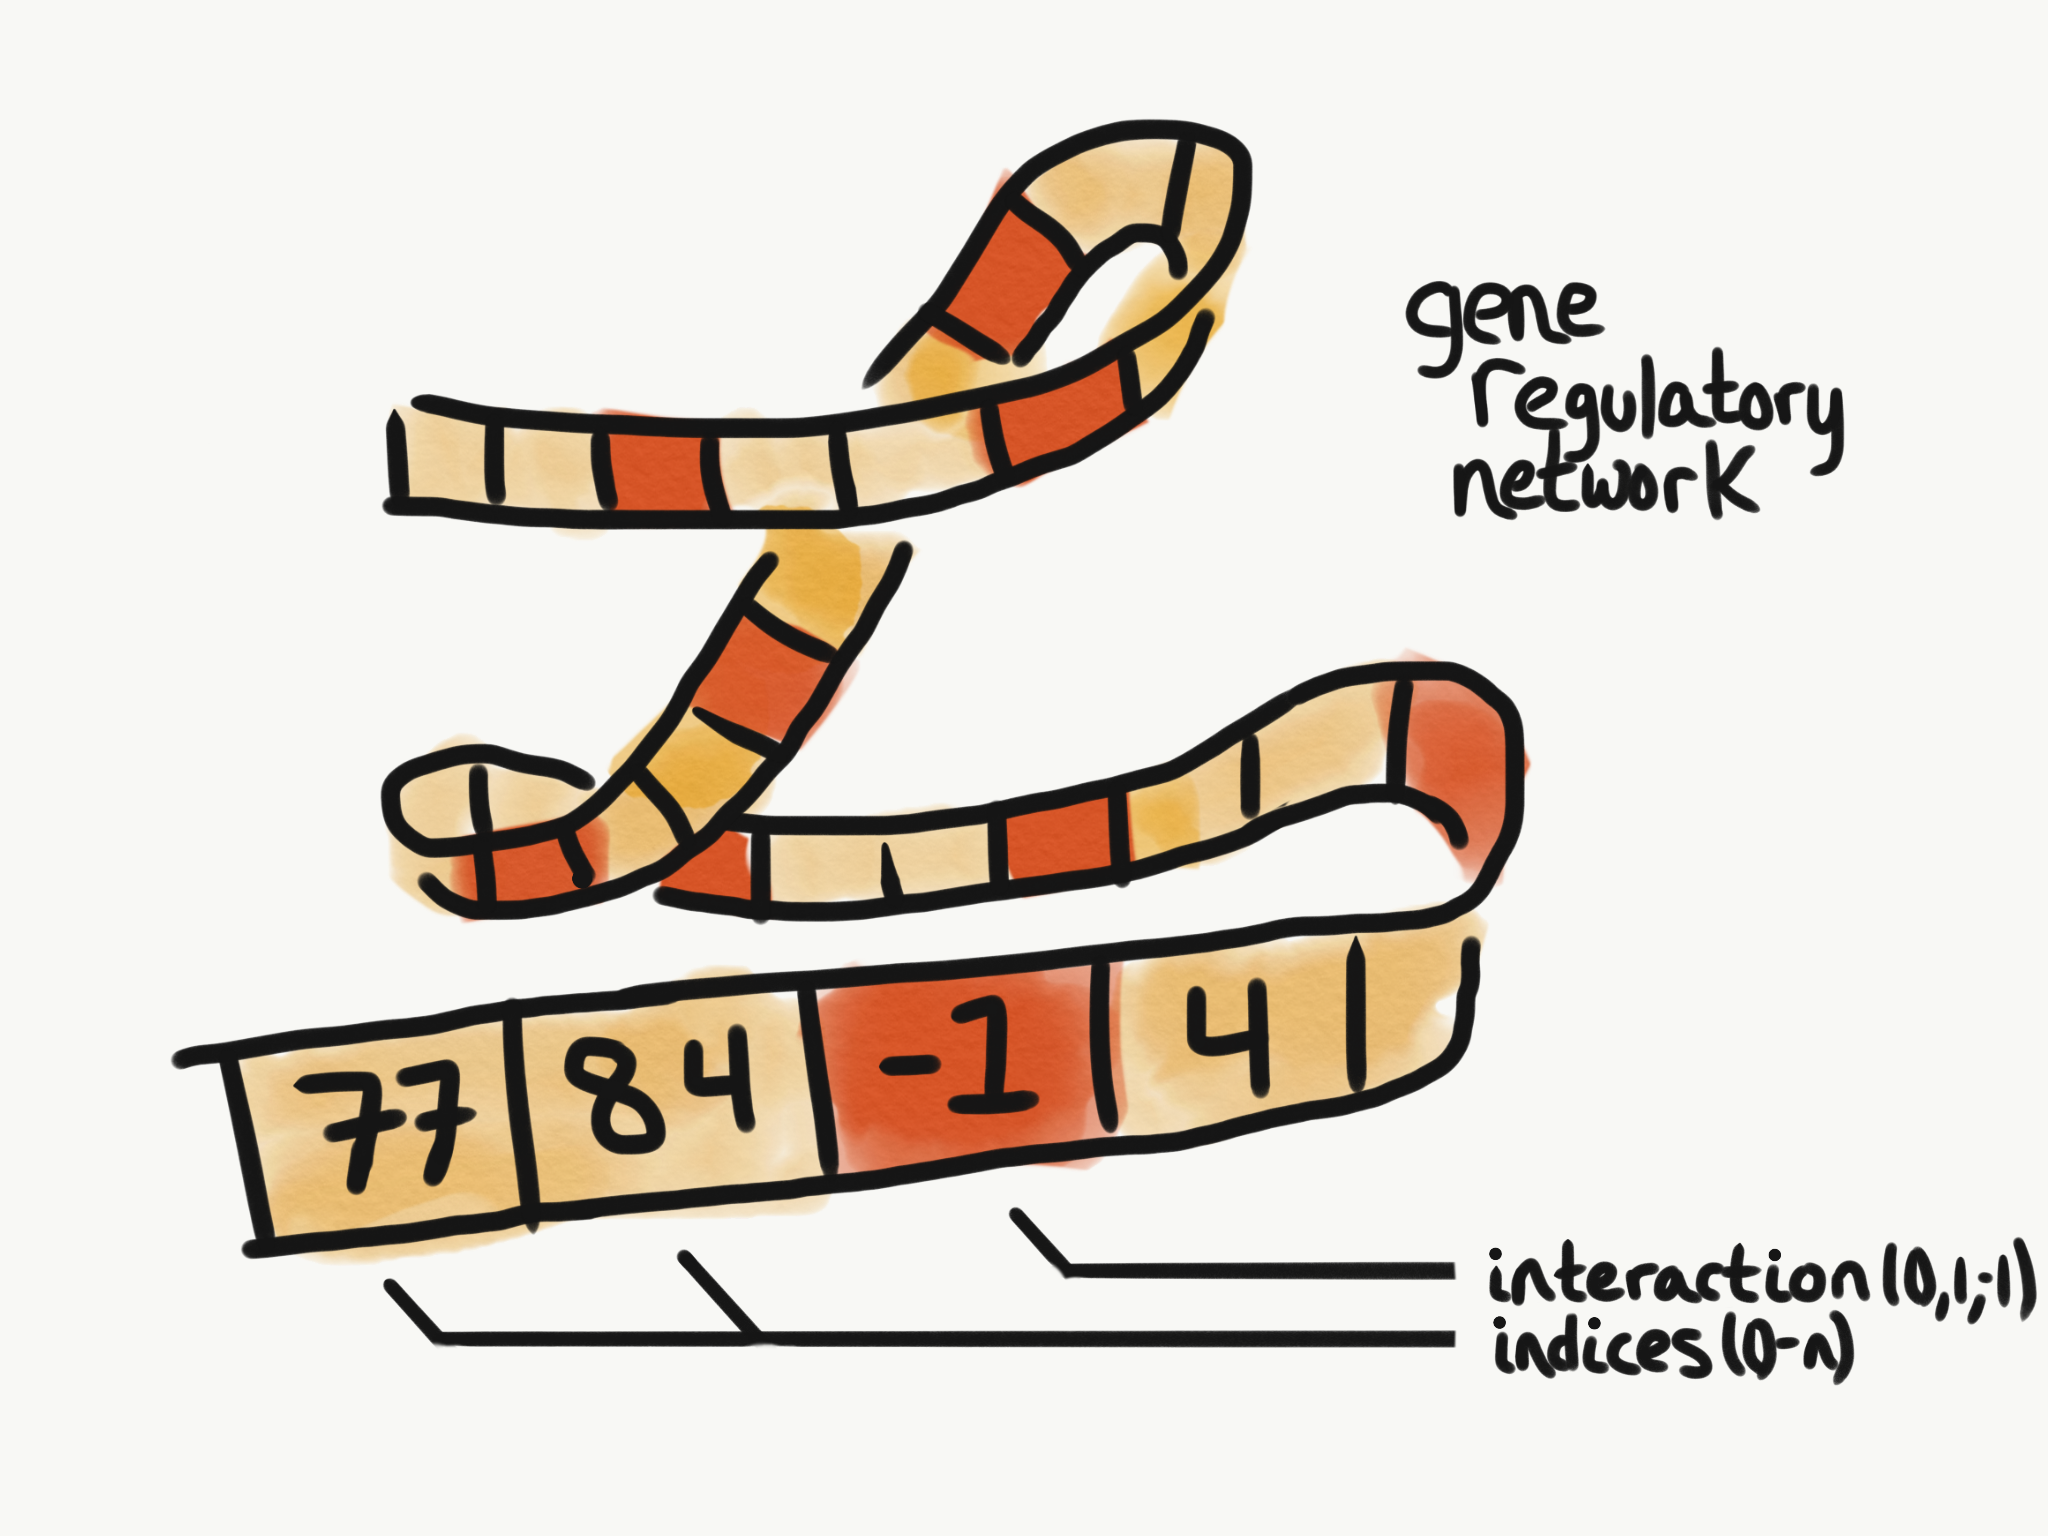
\includegraphics[width=0.8\textwidth]{img/expanded_grn}
 	\captionsetup{singlelinecheck=off,justification=raggedright}
  	\caption{A cartoon depiction of the expanded genetic regulatory network model employed, originally inspired by \cite{Wilder2015ReconcilingEvolvability}.}
    \label{fig:expanded_grn}
\end{figure}
\end{frame}

\begin{frame}{Complete Model}
\begin{figure}
    \centering
    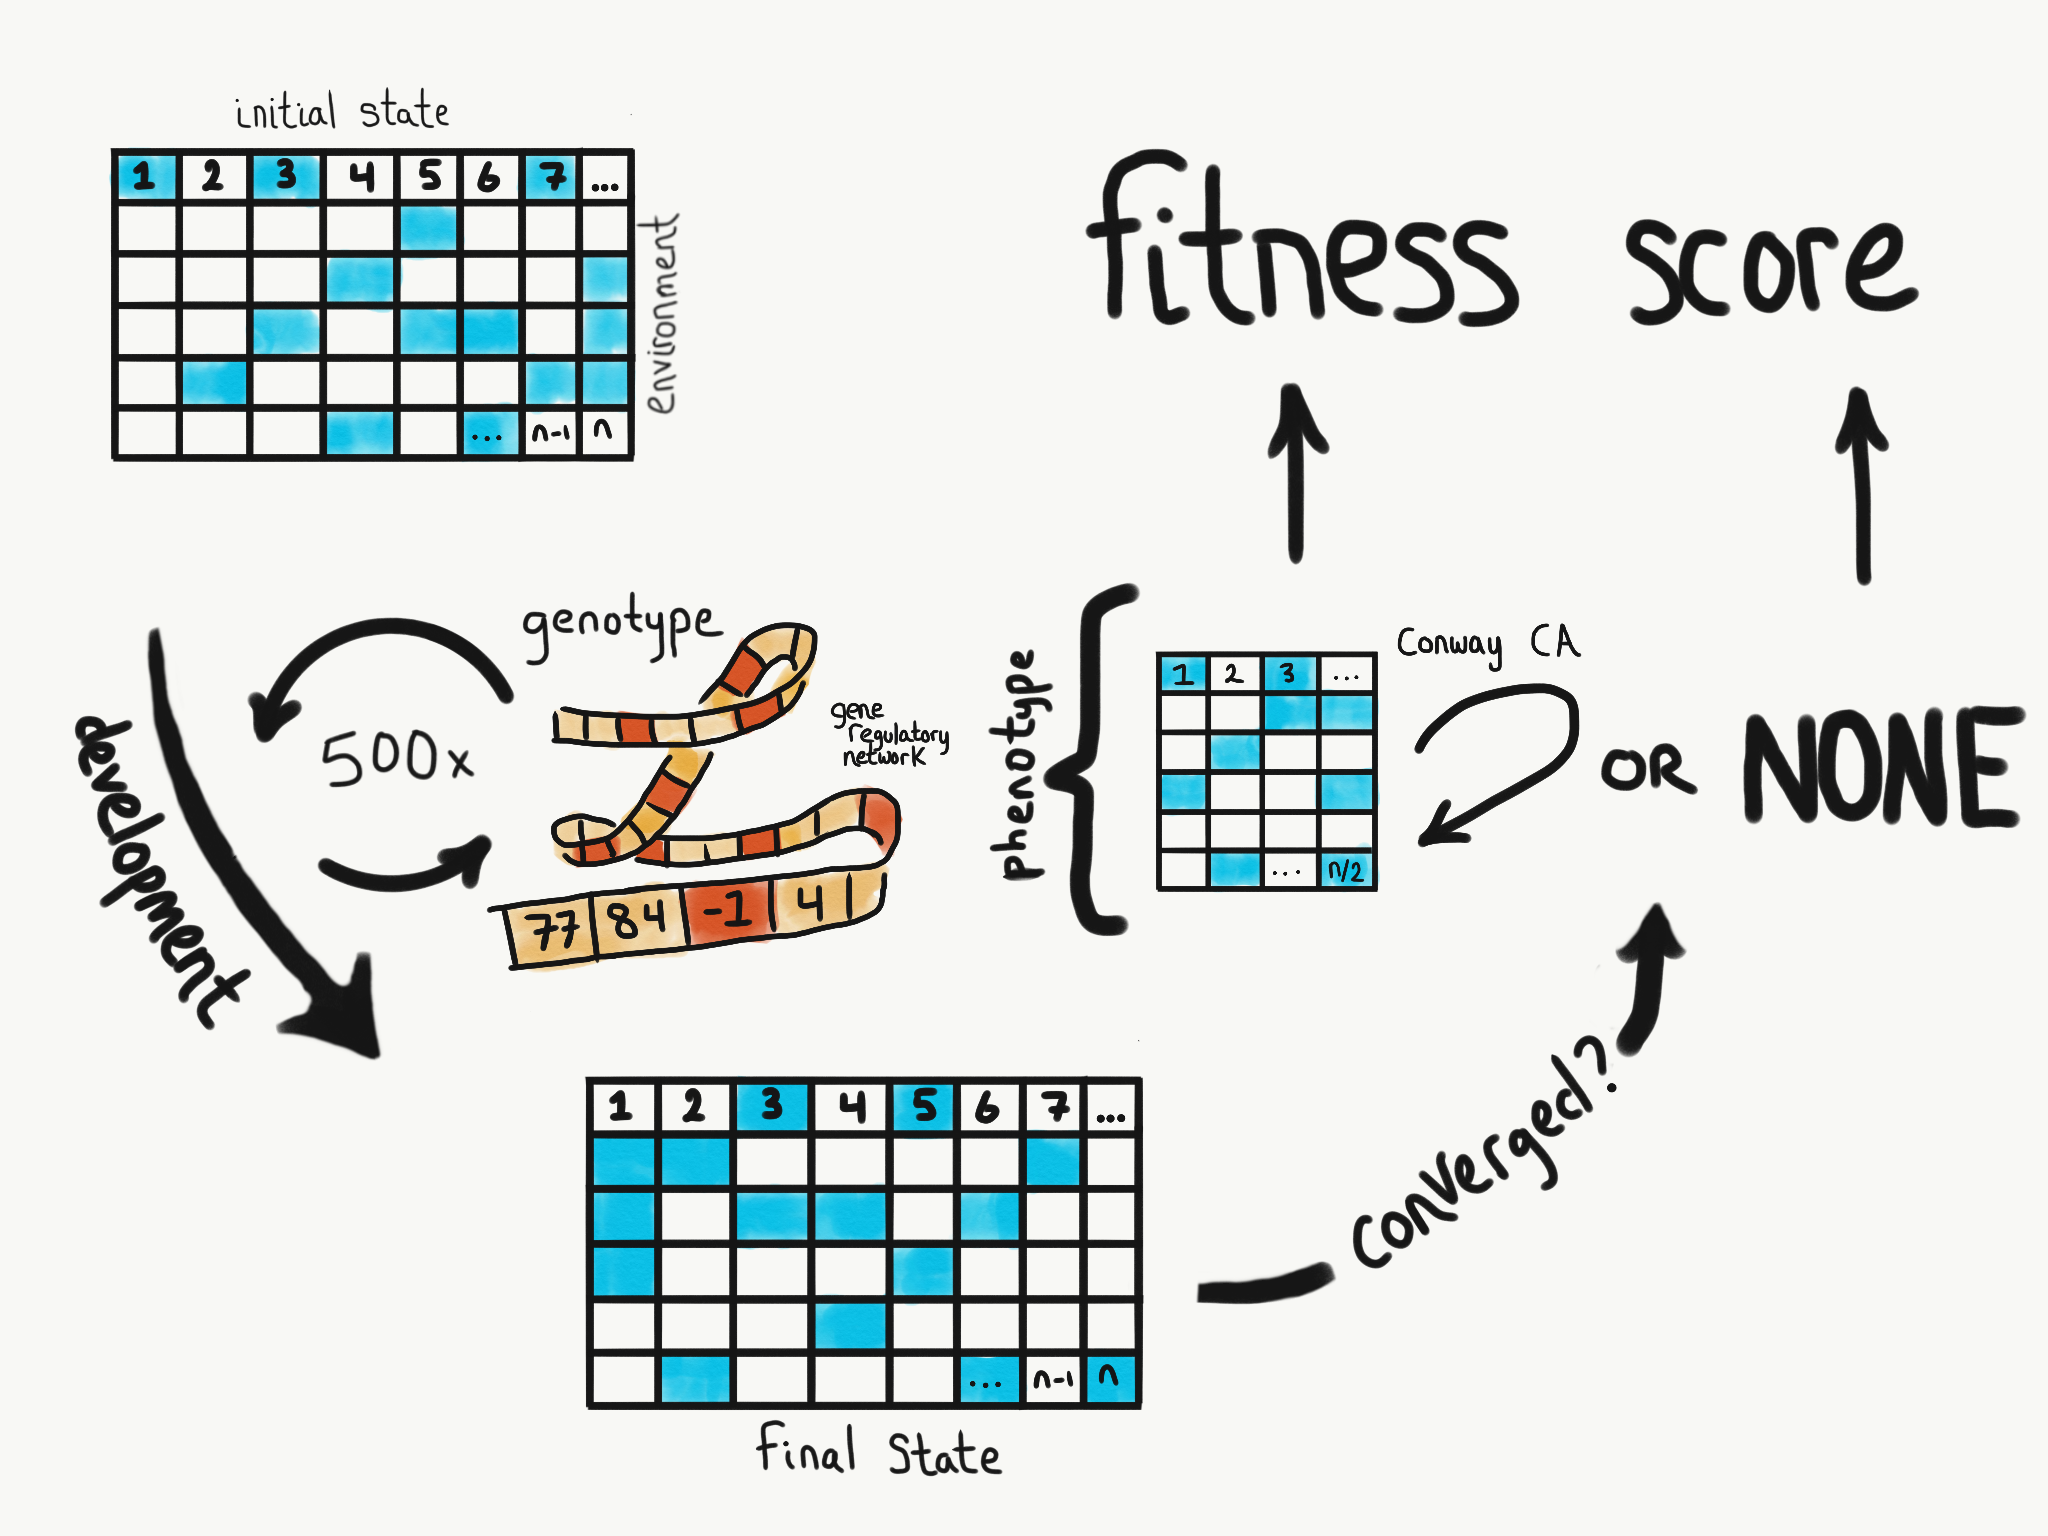
\includegraphics[width=0.8\textwidth]{img/complete_schematic}
 	\captionsetup{singlelinecheck=off,justification=raggedright}
  	\caption{A cartoon overview of the development and assessment processes of the expanded model, based loosely on \cite{Wilder2015ReconcilingEvolvability}.}
    \label{fig:complete_schematic}
\end{figure}
\end{frame}

\begin{frame}{Direct Plasticity: Initial State Perturbation}
\begin{figure}
    \centering
    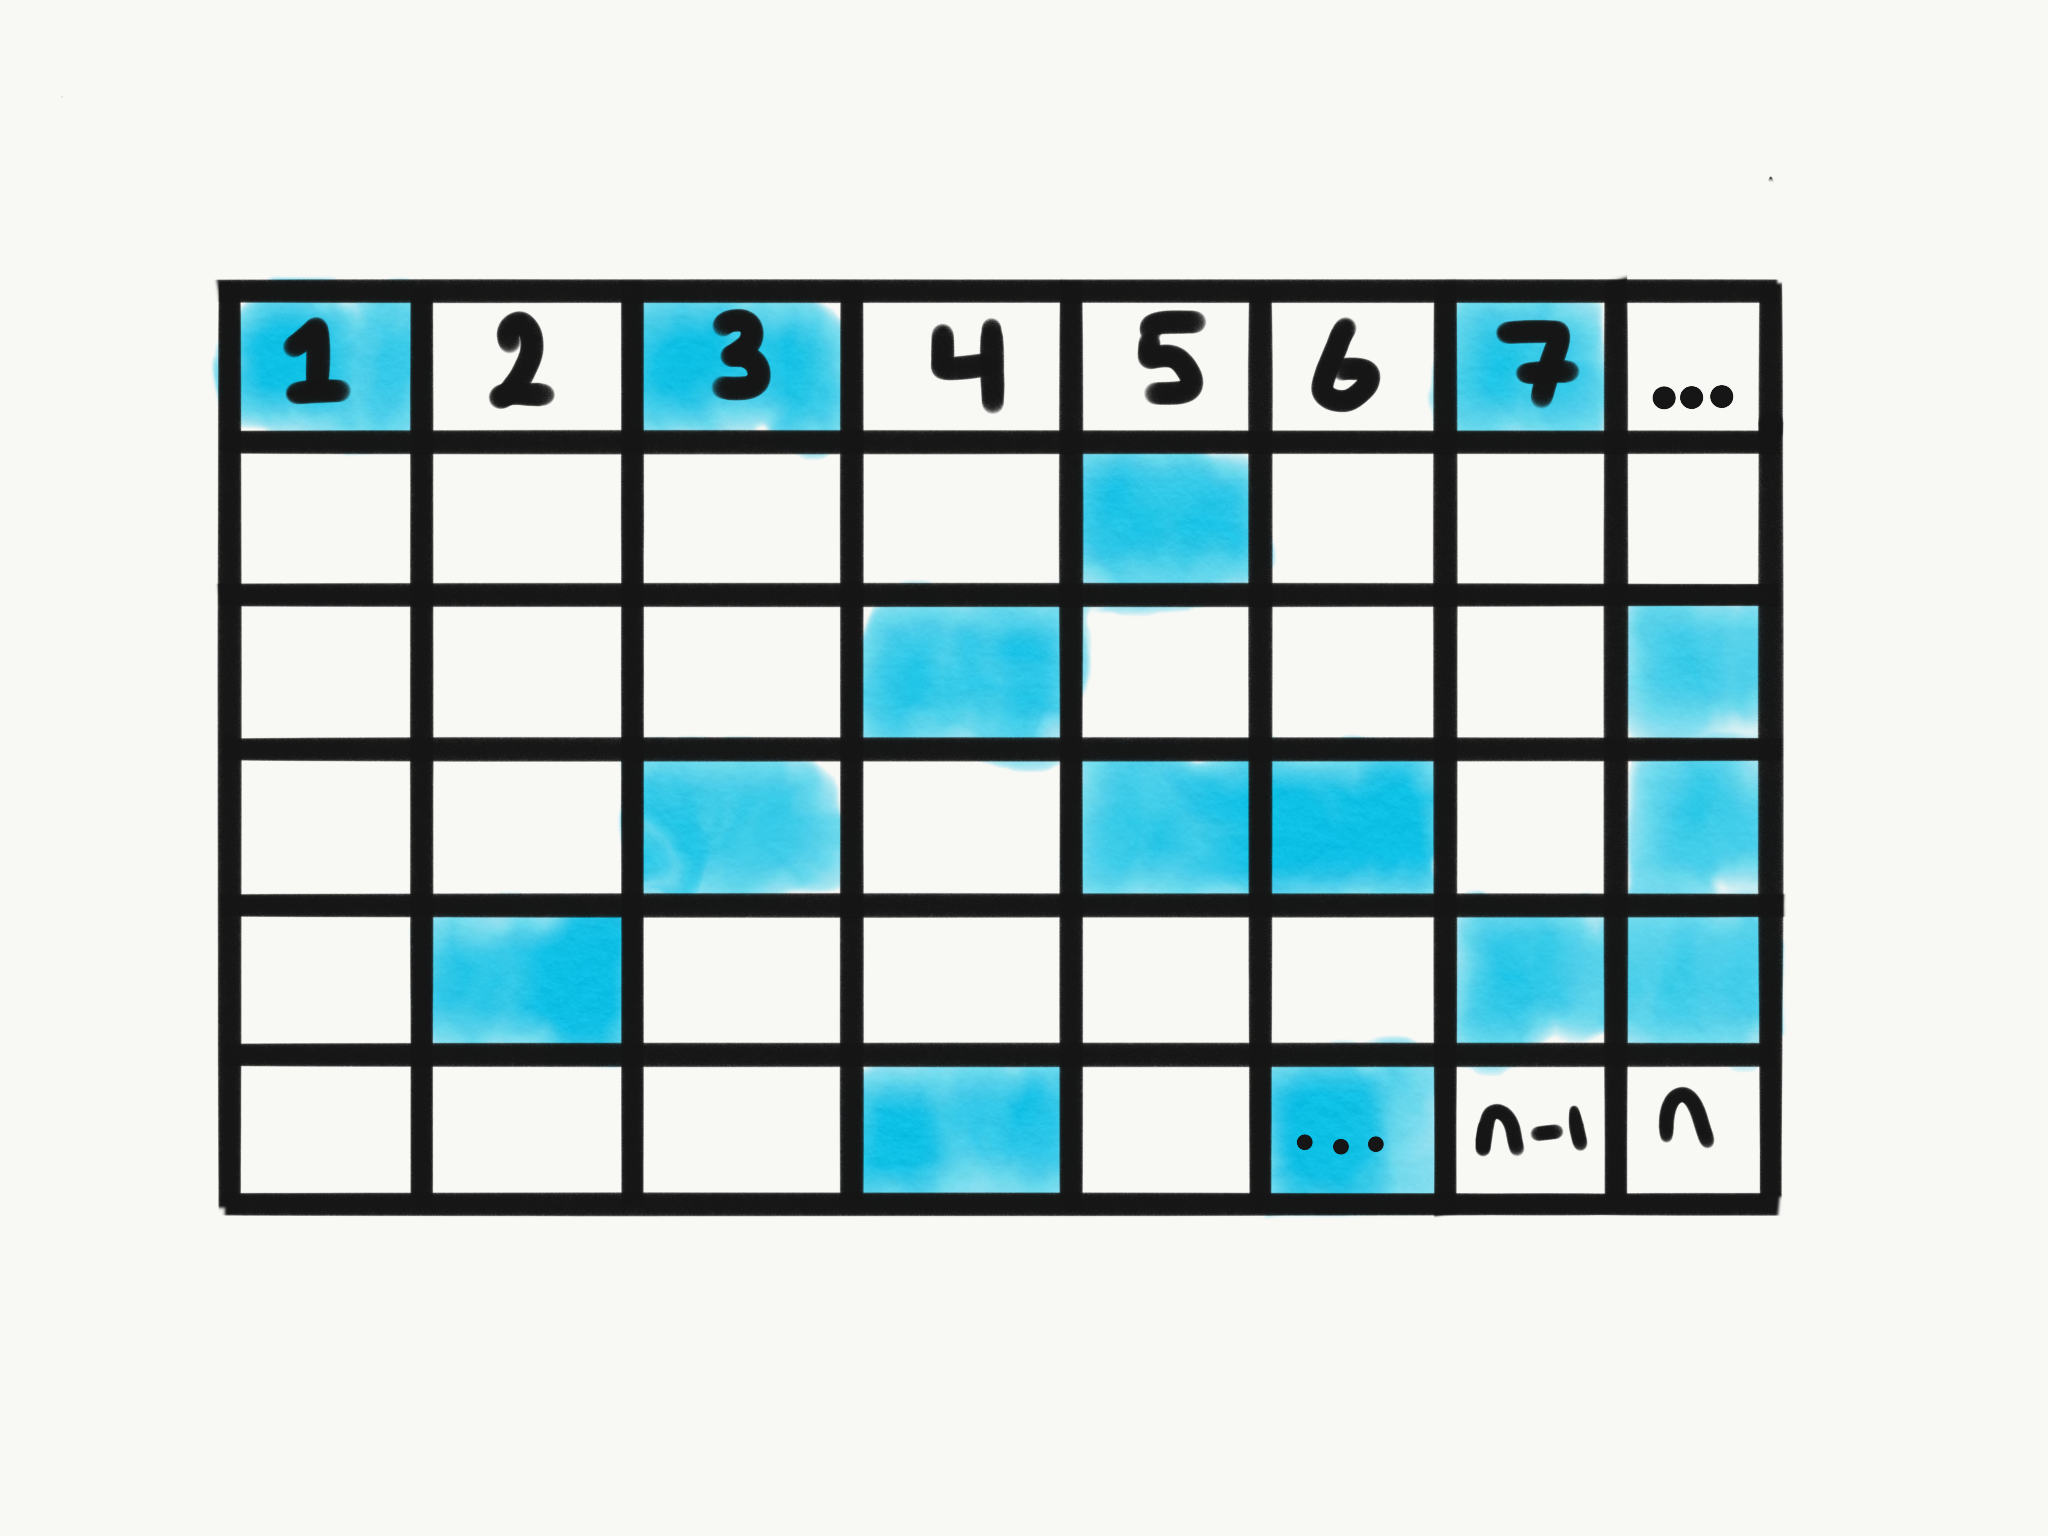
\includegraphics[width=0.8\textwidth]{img/initial_state}
 	\captionsetup{singlelinecheck=off,justification=raggedright}
  	\caption{A graphical example of an initial state, which represents environmental conditions encountered by the genetic regulatory network.}
    \label{fig:initial_state}
\end{figure}
\end{frame}

\begin{frame}{Direct Plasticity: Initial State Perturbation}
\begin{figure}
    \centering
    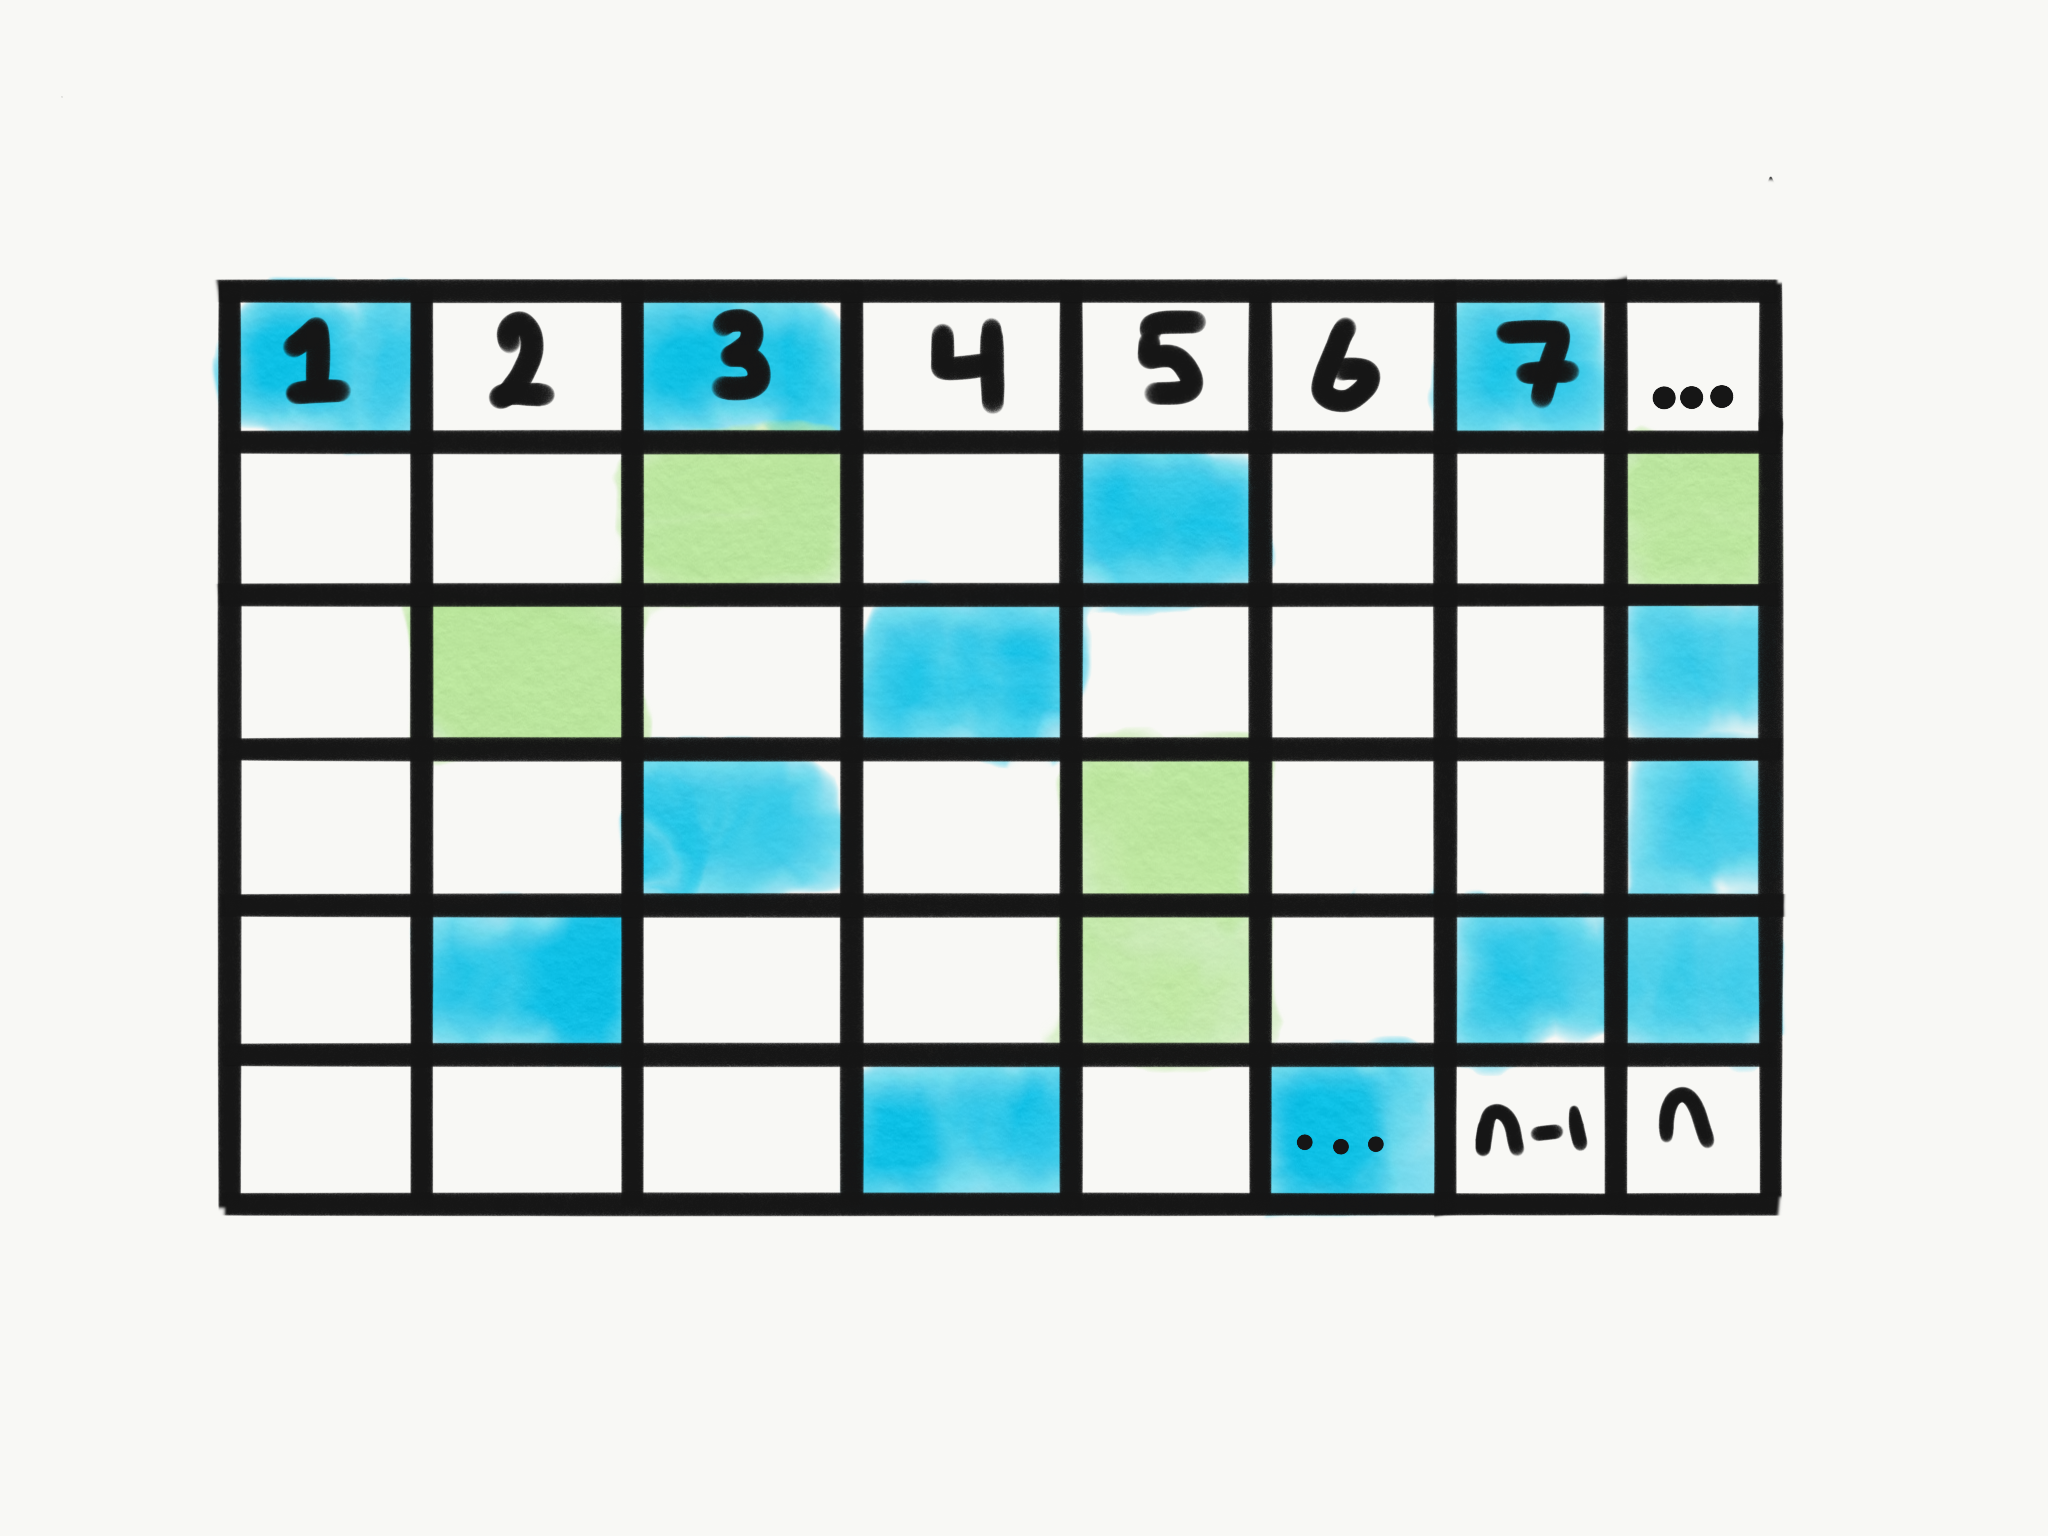
\includegraphics[width=0.8\textwidth]{img/perturbed_initial_state}
 	\captionsetup{singlelinecheck=off,justification=raggedright}
  	\caption{A graphical example of an initial state after random perturbation.}
    \label{fig:perturbed_initial_state}
\end{figure}
\end{frame}

\begin{frame}{Direct Plasticity: Initial State Perturbation}
\begin{figure}
    \centering
    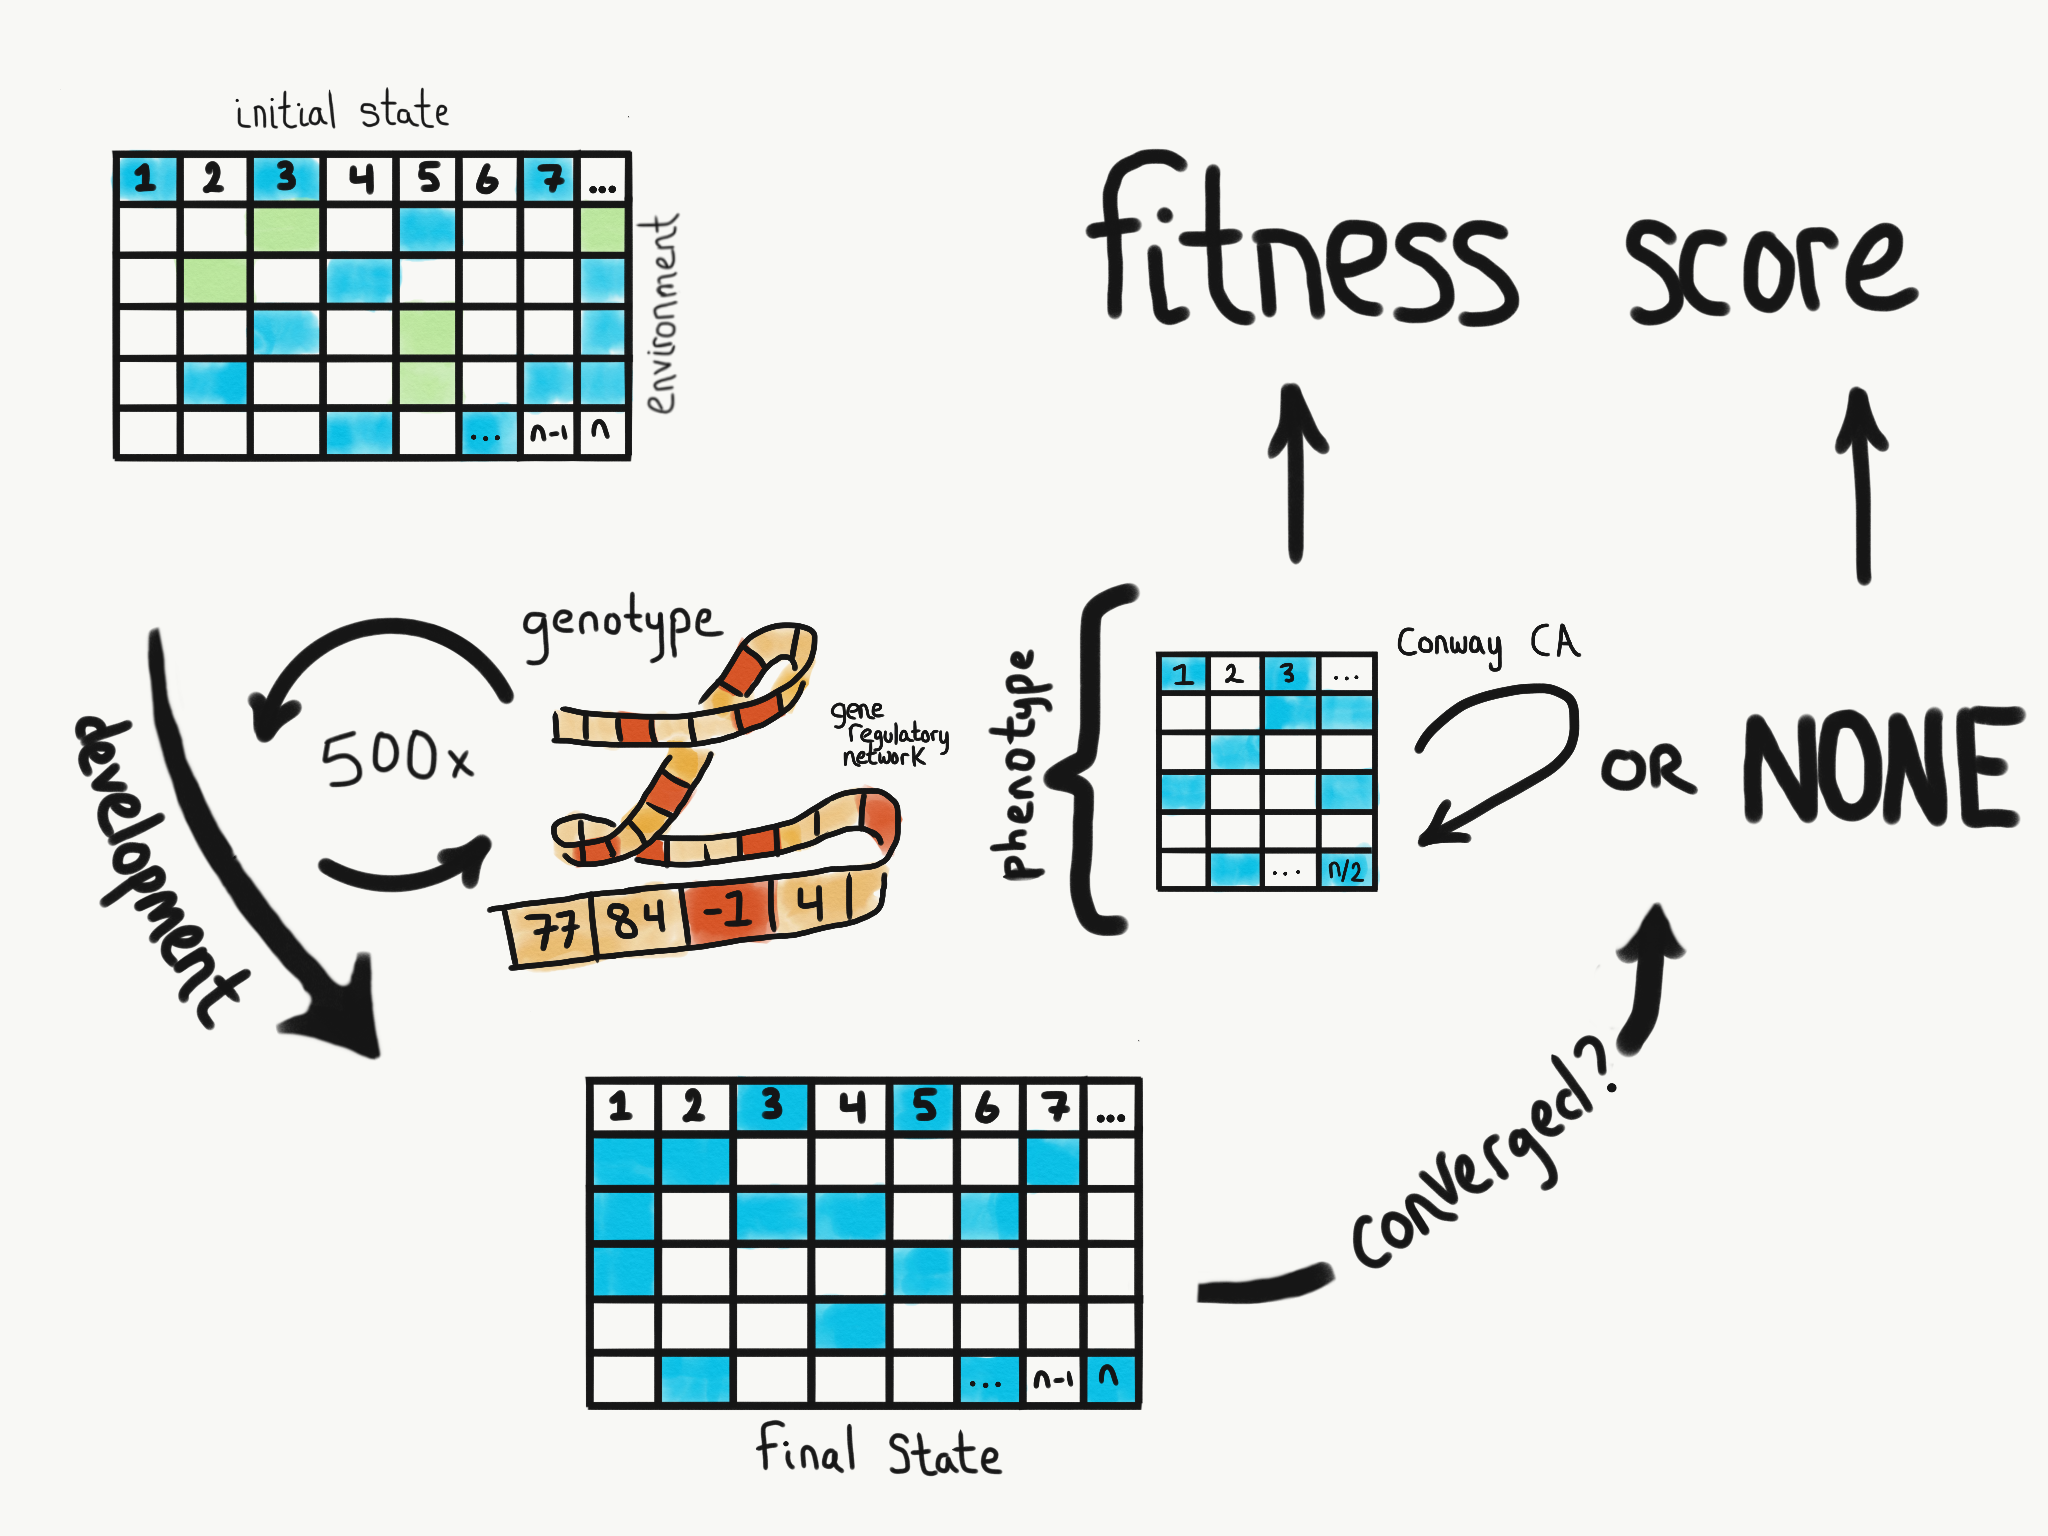
\includegraphics[width=0.8\textwidth]{img/complete_schematic_perturbed}
 	\captionsetup{singlelinecheck=off,justification=raggedright}
  	\caption{A cartoon overview of the development and assessment processes of the expanded model depicting perturbed initial conditions.}
    \label{fig:complete_schematic}
\end{figure}
\end{frame}



\section{Preliminary Results}

\begin{frame}{Evolvability Signature $P=0$}
\begin{figure}
    \centering
    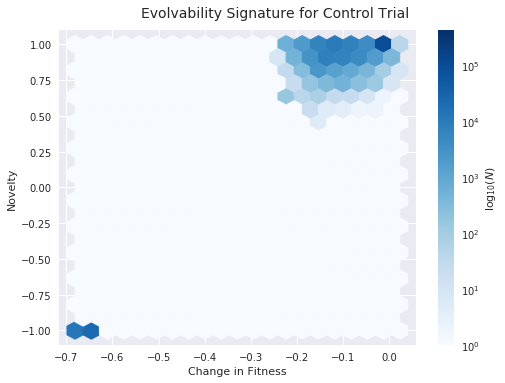
\includegraphics[width=0.8\textwidth]{img/es_p0}
 	\captionsetup{singlelinecheck=off,justification=raggedright}
  	\caption{Evolvability signature of champion evolved with no initial plasticity. Figure after \cite{Tarapore2015EvolvabilityBenchmarks}.}
    \label{fig:es_p0}
\end{figure}
\end{frame}

\begin{frame}{Evolvability Signature $P=0.1$}
\begin{figure}
    \centering
    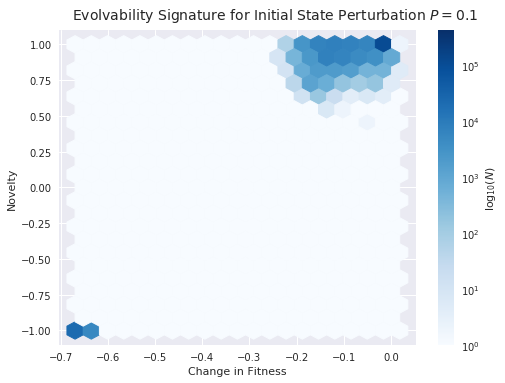
\includegraphics[width=0.8\textwidth]{img/es_p0_1}
 	\captionsetup{singlelinecheck=off,justification=raggedright}
  	\caption{Evolvability signature of champion evolved with medium initial plasticity, $P=0.1$. Figure after \cite{Tarapore2015EvolvabilityBenchmarks}.}
    \label{fig:es_p0_1}
\end{figure}
\end{frame}

\begin{frame}{Evolvability Signature $P=0.2$}
\begin{figure}
    \centering
    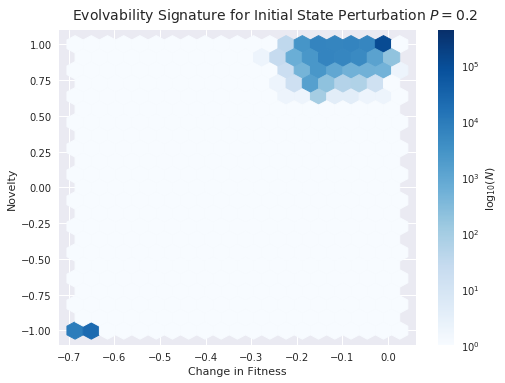
\includegraphics[width=0.8\textwidth]{img/es_p0_2}
 	\captionsetup{singlelinecheck=off,justification=raggedright}
  	\caption{Evolvability signature of champion evolved with greater initial plasticity, $P=0.2$. Figure after \cite{Tarapore2015EvolvabilityBenchmarks}.}
    \label{fig:es_p0_2}
\end{figure}
\end{frame}

\begin{frame}{Frequency of Silent Mutation}
\begin{figure}
    \centering
    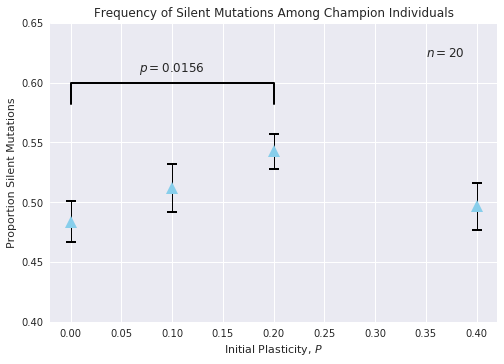
\includegraphics[width=0.8\textwidth]{img/freq_silent_plasticity}
 	\captionsetup{singlelinecheck=off,justification=raggedright}
  	\caption{Frequency of silent mutation of champion individuals across initial plasticity conditions.}
    \label{fig:freq_silent_plasticity}
\end{figure}
\end{frame}

\begin{frame}{Preliminary Results: Summary}
\begin{itemize}
  \item as in \cite{Reisinger2005TowardsEvolvability}, repeated evaluations ($n=10$) were required to observe impact of direct plasticity
  \item direct plasticity increases robustness to mutation
  \item direct plasticity does not seem to promote canalization 
\end{itemize}
\end{frame}

\section{Project Schedule}

\begin{frame}{Experimental Questions}
\begin{itemize}
\item how do genetic regulatory networks evolved with direct plasticity differ structurally from control networks? \cite{Reisinger2007AcquiringRepresentations}
\item impact of other modes of direct plasticity on evolvability (rule noise, fixed states, intermediate state perturbation)?
\item impact of indirect plasticity on evolvability?   
\item combined impact of direct and indirect plasticity on evolvability?   
\end{itemize}
\end{frame}

\begin{frame}{Progress To Date}
\begin{center}
{\centering ~$\bm{\vdots}$~}
\end{center}
\begin{itemize}
  \item \textbf{Week 5} -- code and test second model (part III) \checkmark
  \item \textbf{Week 6} -- run second model \checkmark
  \item \textbf{Week 7} -- analyze data from second model \checkmark
  \item \textbf{Week 8} -- further experimental tweaks and data collection \checkmark
  \item \textbf{Week 9} -- spring break, complete data collection \ding{55}
\end{itemize}
\vspace{-1ex}
\begin{center}
{\centering ~$\bm{\vdots}$~}
\end{center}
\end{frame}

\begin{frame}{From Here Onwards (old plan)}
\begin{center}
{\centering ~$\bm{\vdots}$~}
\end{center}
\begin{itemize}
 \item \textbf{Week 10}
  \begin{itemize}
    \item \textit{Wednesday March 22nd}: Honors thesis presentation
  \end{itemize}
  \item \textbf{Week 11} prepare for departmental presentation, Complete data analysis
  \item \textbf{Week 12} thesis writing \Coffeecup \Coffeecup \Coffeecup
  \begin{itemize}
    \item \textit{Monday April 3rd}: Math/CS Department seminar
  \end{itemize}
  \item \textbf{Week 13}  more, and more frantic, thesis writing \Coffeecup \Coffeecup \Coffeecup \Coffeecup \Coffeecup
  \item \textbf{Week 14} prepare for Math/CS Day presentation, adapt thesis material for Capstone report
  \item \textbf{Week 15} prepare for Math/CS Day presentation, adapt thesis material for Capstone report
  \begin{itemize}
  	\item \textit{Saturday April 29th}: Math/CS Day presentation
  \end{itemize}
 \end{itemize}
\vspace{-1ex}
\begin{center}
{\centering ~$\bm{\vdots}$~}
\end{center}
\end{frame}

\begin{frame}{From Here Onwards (new plan)}
\begin{center}
{\centering ~$\bm{\vdots}$~}
\end{center}
\begin{itemize}
 \item \textbf{Week 10} perform experiments with indirect plasticity
  \item \textbf{Week 11} perform experiments with indirect plasticity
  \item \textbf{Week 12} perform combined experiments with indirect and direct plasticity
  \item \textbf{Week 13} network structure analysis
  \begin{itemize}
    \item \textit{Monday April 10th}: Math/CS Department presentation
  \end{itemize}
  \item \textbf{Week 14} prepare for Math/CS Day presentation, capstone writeup
  \item \textbf{Week 15} prepare for Math/CS Day presentation, capstone writeup
  \begin{itemize}
  	\item \textit{Saturday April 29th}: Math/CS Day presentation
  \end{itemize}
 \end{itemize}
\vspace{-1ex}
\begin{center}
{\centering ~$\bm{\vdots}$~}
\end{center}
\end{frame}

\appendix


\begin{frame}[standout]
  Questions?
\end{frame}

\begin{frame}[allowframebreaks]{References}

  \bibliography{Mendeley}
  \setbeamertemplate{bibliography item}{\insertbiblabel}
  %\nocite{*} % Insert publications even if they are not cited in the poster
  \bibliographystyle{apalike}
\end{frame}

\begin{frame}{Frequency of Nondeleterious Mutation}
\begin{figure}
    \centering
    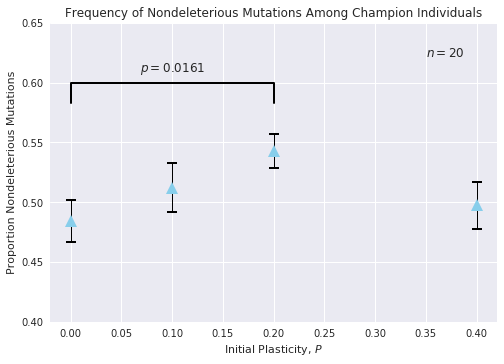
\includegraphics[width=0.8\textwidth]{img/freq_nondeleterious_plastic}
 	\captionsetup{singlelinecheck=off,justification=raggedright}
  	\caption{Frequency of nondeleterious mutation of champion individuals across initial plasticity conditions.}
    \label{fig:freq_nondeleterious_plastic}
\end{figure}
\end{frame}



\end{document}
